
\documentclass[11 pt,t]{beamer}
\usepackage{verbatim}
\usepackage{latexsym}
\usepackage{amsmath,amsfonts,amssymb}
\usepackage{algorithmicx,algorithm}
\usepackage{amsfonts,amssymb}
\graphicspath{{figures/}}    
\usetheme[
	bullet=circle,		% Other option: square
	bigpagenumber,		% circled page number on lower right
	topline=true,		% colored bar at the top of the frame 
	]{Zurich}

\tikzstyle{decision} = [diamond, draw, fill=blue!20,
text width=4.5em, text badly centered, node distance=3cm, inner sep=0pt]
\tikzstyle{block} = [rectangle, draw, fill=blue!20,
text width=5em, text centered, rounded corners, minimum height=4em]
\tikzstyle{line} = [draw, -latex']
\tikzstyle{cloud} = [draw, ellipse,fill=red!20, node distance=3cm,
    minimum height=2em]
\usetikzlibrary{arrows}
\usetikzlibrary{decorations.pathreplacing}
\makeatletter
% add a macro that saves its argument
\newcommand{\footlineextra}[1]{\gdef\insertfootlineextra{#1}}
\newbox\footlineextrabox
 
% add a beamer template that sets the saved argument in a box.
% The * means that the beamer font and color "footline extra" are automatically added. 
\defbeamertemplate*{footline extra}{default}{
  \begin{beamercolorbox}[ht=2.25ex,dp=1ex,leftskip=\Gm@lmargin]{footline extra}
    \insertfootlineextra
    % \par\vspace{2.5pt}
  \end{beamercolorbox}
}
 
\addtobeamertemplate{footline}{%
  % set the box with the extra footline material but make it add no vertical space
  \setbox\footlineextrabox=\vbox{\usebeamertemplate*{footline extra}}
  \vskip -\ht\footlineextrabox
  \vskip -\dp\footlineextrabox
  \box\footlineextrabox%
}
{}
 
% patch \begin{frame} to reset the footline extra material
\let\beamer@original@frame=\frame
\def\frame{\gdef\insertfootlineextra{}\beamer@original@frame}
\footlineextra{}
\makeatother
%-----------------------------------------------------------------------------
% DOCUMENT PROPERTIES
\logo{
\includegraphics[scale=0.13]{ouclogo.png}}
\author{DingHao}
\title{Research of Histogram}

%-----------------------------------------------------------------------------


\begin{document}


% ----------------------------------------------------------------------------
\frame{\titlepage}
\frame{\frametitle{Contents}\tableofcontents}
% ----------------------------------------------------------------------------


\section{Histogram Equalization}
\subsection{Task}

\begin{frame}
\frametitle{Histogram Equalization}
\framesubtitle{Task}
Choose a grayscale image\\
\begin{block}{1)}
   applying global histogram equalization(HE) to it
\end{block}
\begin{block}{2)}
   applying adaptive histogram equalization(AHE) to the image and try to exchange the size of topical blocks
\end{block}
\begin{block}{3)}
   disscuss the results
\end{block}
\end{frame}

\subsection{Introduction}

\begin{frame}
\frametitle{Histogram Equalization}
\framesubtitle{Introduction}
\vspace{6pt}
\begin{itemize}
\item Histogram: straggling probability density distribution
\vspace{6pt}
\item Histogram equalization: using justify space between grayscales
\vspace{6pt}
\begin{itemize}
\item[-] dynamic histogram equalization
\item[-] global histogram equalization(HE)
\item[-] adaptive histogram equalization(AHE)
\item[-] contrast-limited adaptive histogram equalization(CLAHE)
\item[-] bilinear interpolation
\item[-] histogram normalization
\end{itemize}
\end{itemize}
\end{frame}

\subsection{Method}

\begin{frame}
\frametitle{Method}
\framesubtitle{HE}

\begin{table}[!ht]
%\centering
\toprule
\begin{tabular}{l p{.88\linewidth}}
\vspace{6pt}
1. draw the histogram $p_{r}\left(r_{k}\right)=\frac{n_{k}}{N}$\\
\vspace{6pt}
2. calculate the integral histogram $s_{k}'=T\left(r_{k}\right)=\sum^{k}_{j=0}p_{r}\left(r_{j}\right)$\\
\vspace{6pt}
3. multiply the integral histogram by 255 $s_{k}=\left(L-1\right)s_{k}'$\\
\vspace{6pt}
4. the result is the output
\end{tabular}
\end{table}
\end{frame}

\begin{frame}
\frametitle{Method}
\framesubtitle{HE}
\begin{minipage}[t]{\linewidth}\centering
\vspace{12pt}
\begin{figure}
   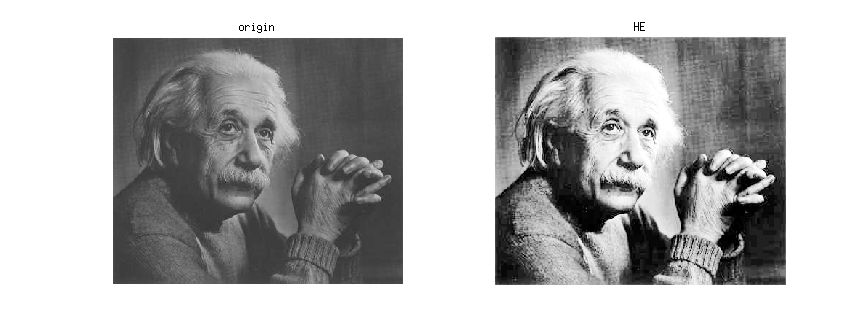
\includegraphics[width=10cm]{HEeinstein.png}
\end{figure}
\end{minipage}
\end{frame}

\begin{frame}
\frametitle{Method}
\framesubtitle{AHE}
\vspace{20pt}
\begin{center}
AHE is the rigional HE
\end{center}
\end{frame}


\begin{frame}
\frametitle{Method}
\framesubtitle{AHE}
\begin{minipage}[t]{\linewidth}\centering
\begin{figure}
   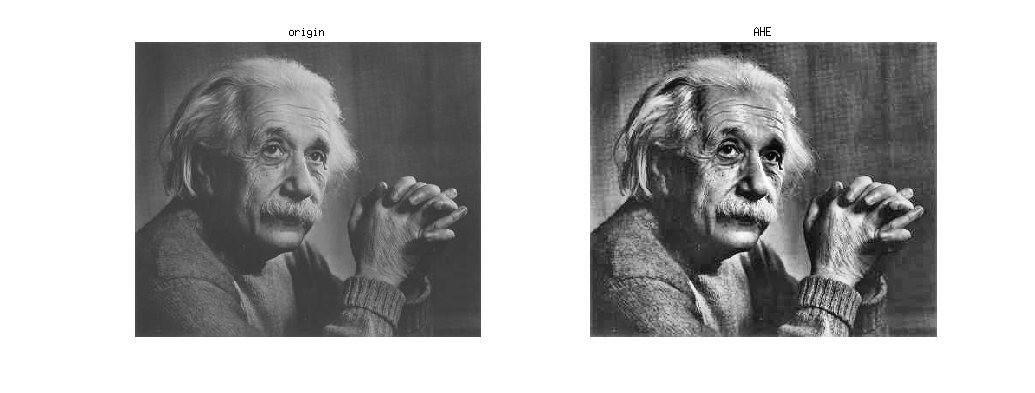
\includegraphics[width=8cm]{AHEeinstein.png}
\end{figure}
\end{minipage}
\end{frame}

\begin{frame}
\frametitle{Method}
\framesubtitle{CLAHE}
\vspace{20pt}
\begin{center}
limit noise amplification
\end{center}
\end{frame}


\begin{frame}
\frametitle{Method}
\framesubtitle{CLAHE}
\begin{minipage}[t]{\linewidth}\centering
\begin{figure}
   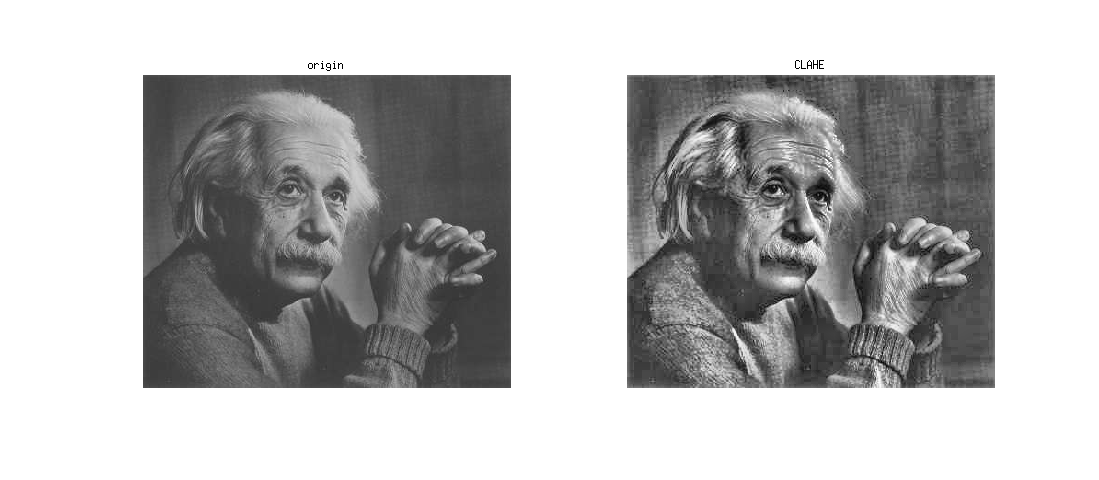
\includegraphics[width=8cm]{CLAHEeinstein.png}
\end{figure}
\end{minipage}
\end{frame}

\subsection{Result}

\begin{frame}
\frametitle{Result}
\framesubtitle{Different images}
\begin{minipage}[t]{\linewidth}\centering
\begin{figure}
   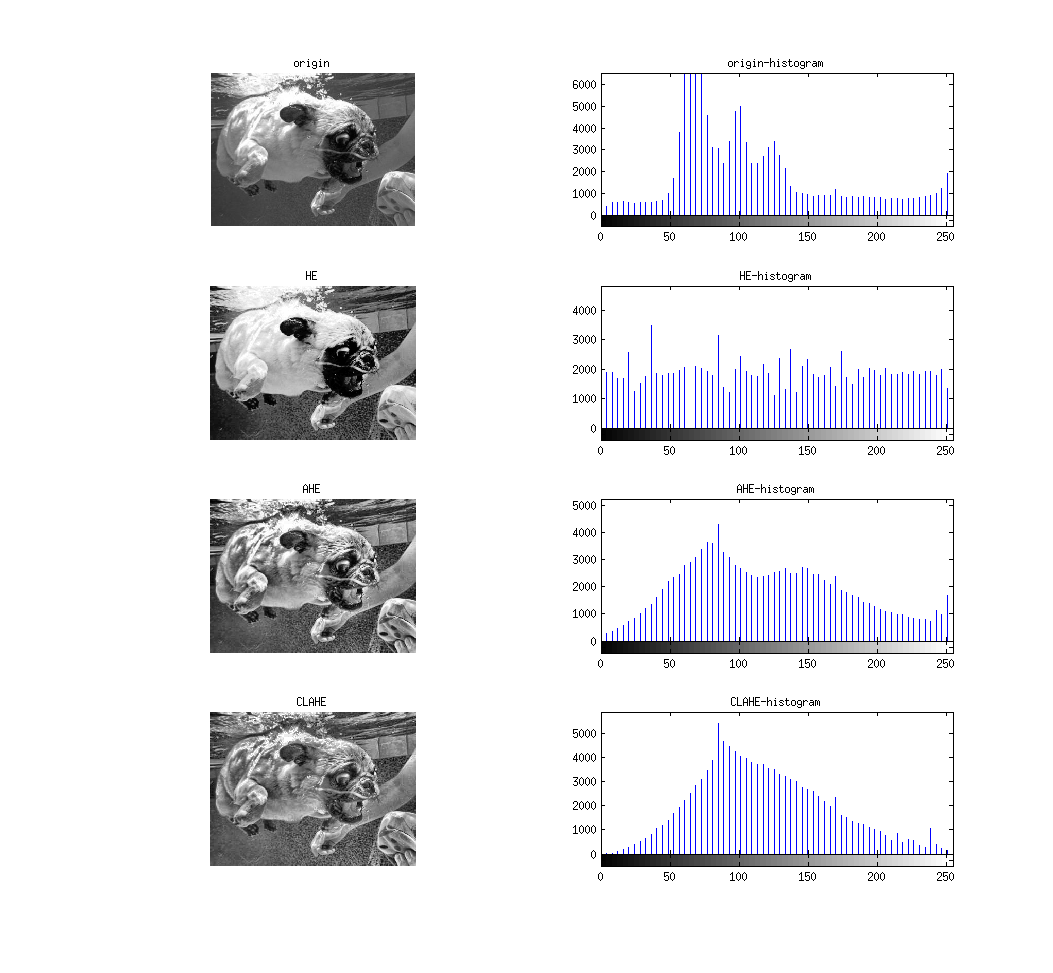
\includegraphics[width=8.5cm]{dog.png}
\end{figure}
\end{minipage}
\end{frame}
%\begin{block}{ZooScan}
 %  427 / 28 = 15.25
%\end{block}
%\begin{exampleblock}{Kaggle}
%   1979 / 9 = 219.89
%\end{exampleblock}
%\begin{alertblock}{WHOI}
%   2606720 / 4 = 651680
%\end{alertblock}
%{\textcolor{tangocolordarkchameleon}{EVEN MORE THAN $10^{8}$ !} }
\begin{frame}
\frametitle{Result}
\framesubtitle{Different images}
\begin{minipage}[t]{\linewidth}\centering
\begin{figure}
   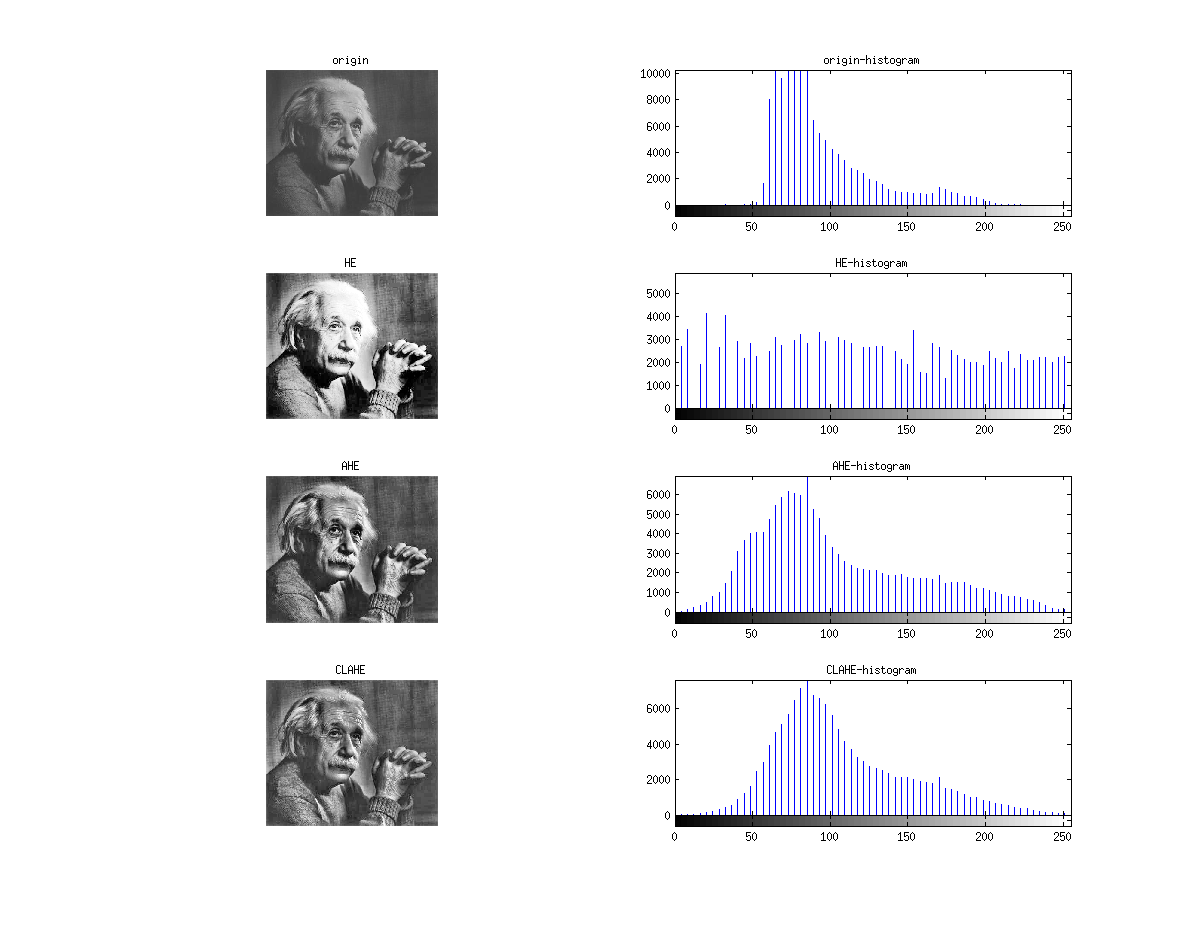
\includegraphics[width=10cm]{einstein.png}
\end{figure}
\end{minipage}
\end{frame}

%\begin{center}%\begin{minipage}[t]{\linewidth}\centering
%\Huge{WHY?}
%\end{minipage}
%\end{center}
\begin{frame}
\frametitle{Result}
\framesubtitle{Size of blocks}
\begin{minipage}[t]{\linewidth}\centering
\begin{figure}
   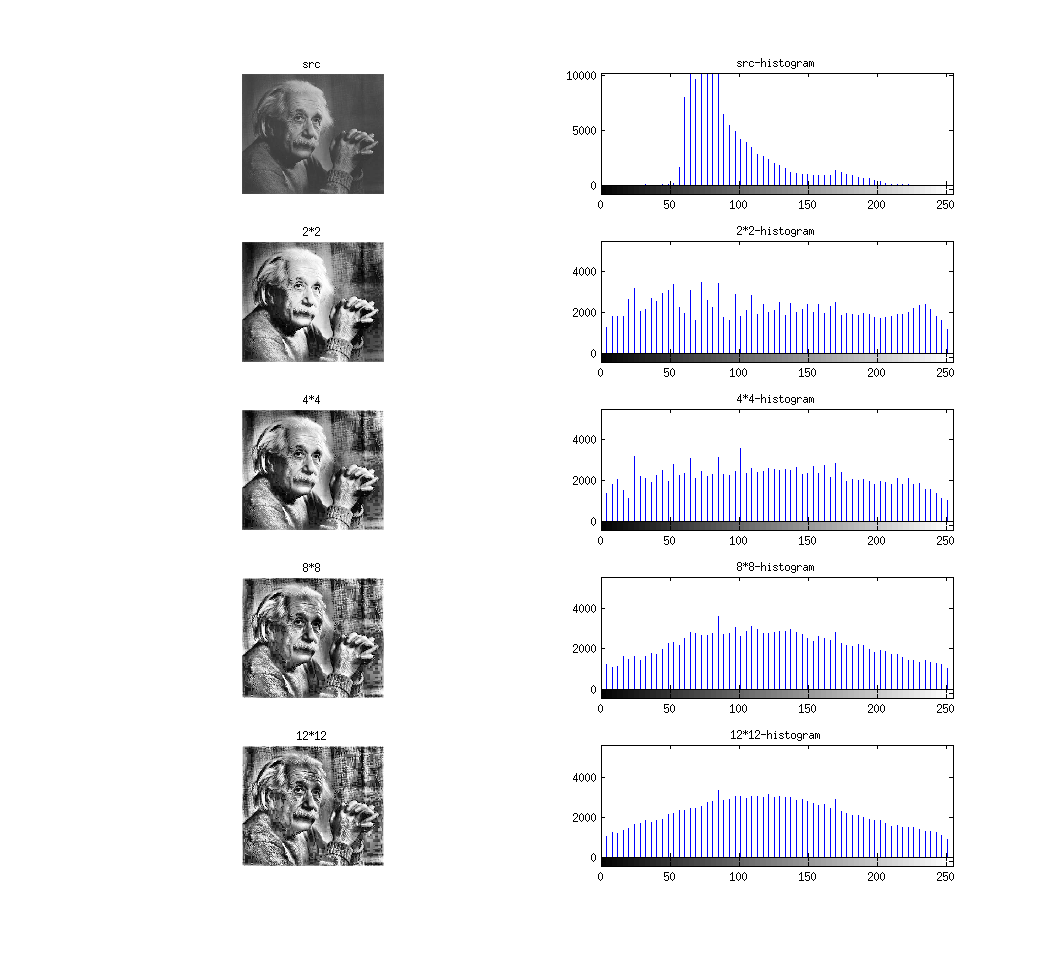
\includegraphics[width=8cm]{block.png}
\end{figure}
\end{minipage}
\end{frame}

\begin{frame}
\frametitle{Result}
\framesubtitle{Histogram normalization}
\begin{minipage}[t]{\linewidth}\centering
\begin{figure}
   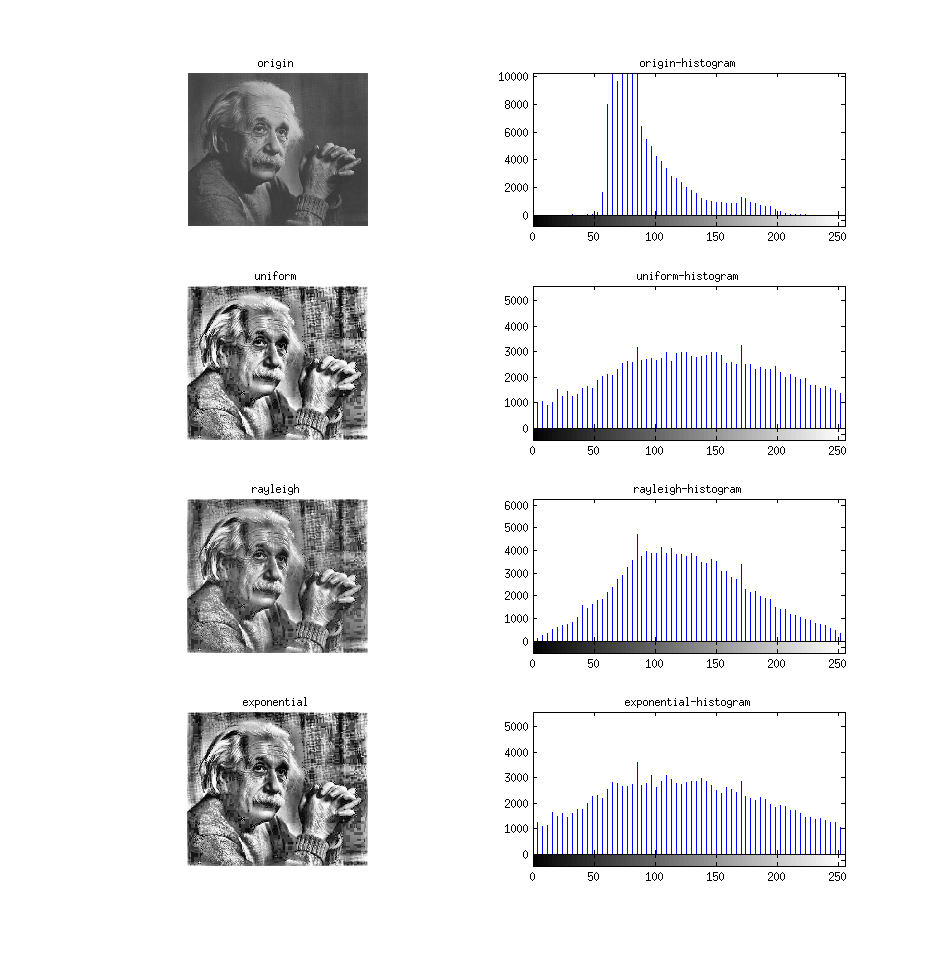
\includegraphics[width=8cm]{distribution.png}
\end{figure}
\end{minipage}
\end{frame}


% ----------------------------------------------------------------------------
\usebackgroundtemplate{
   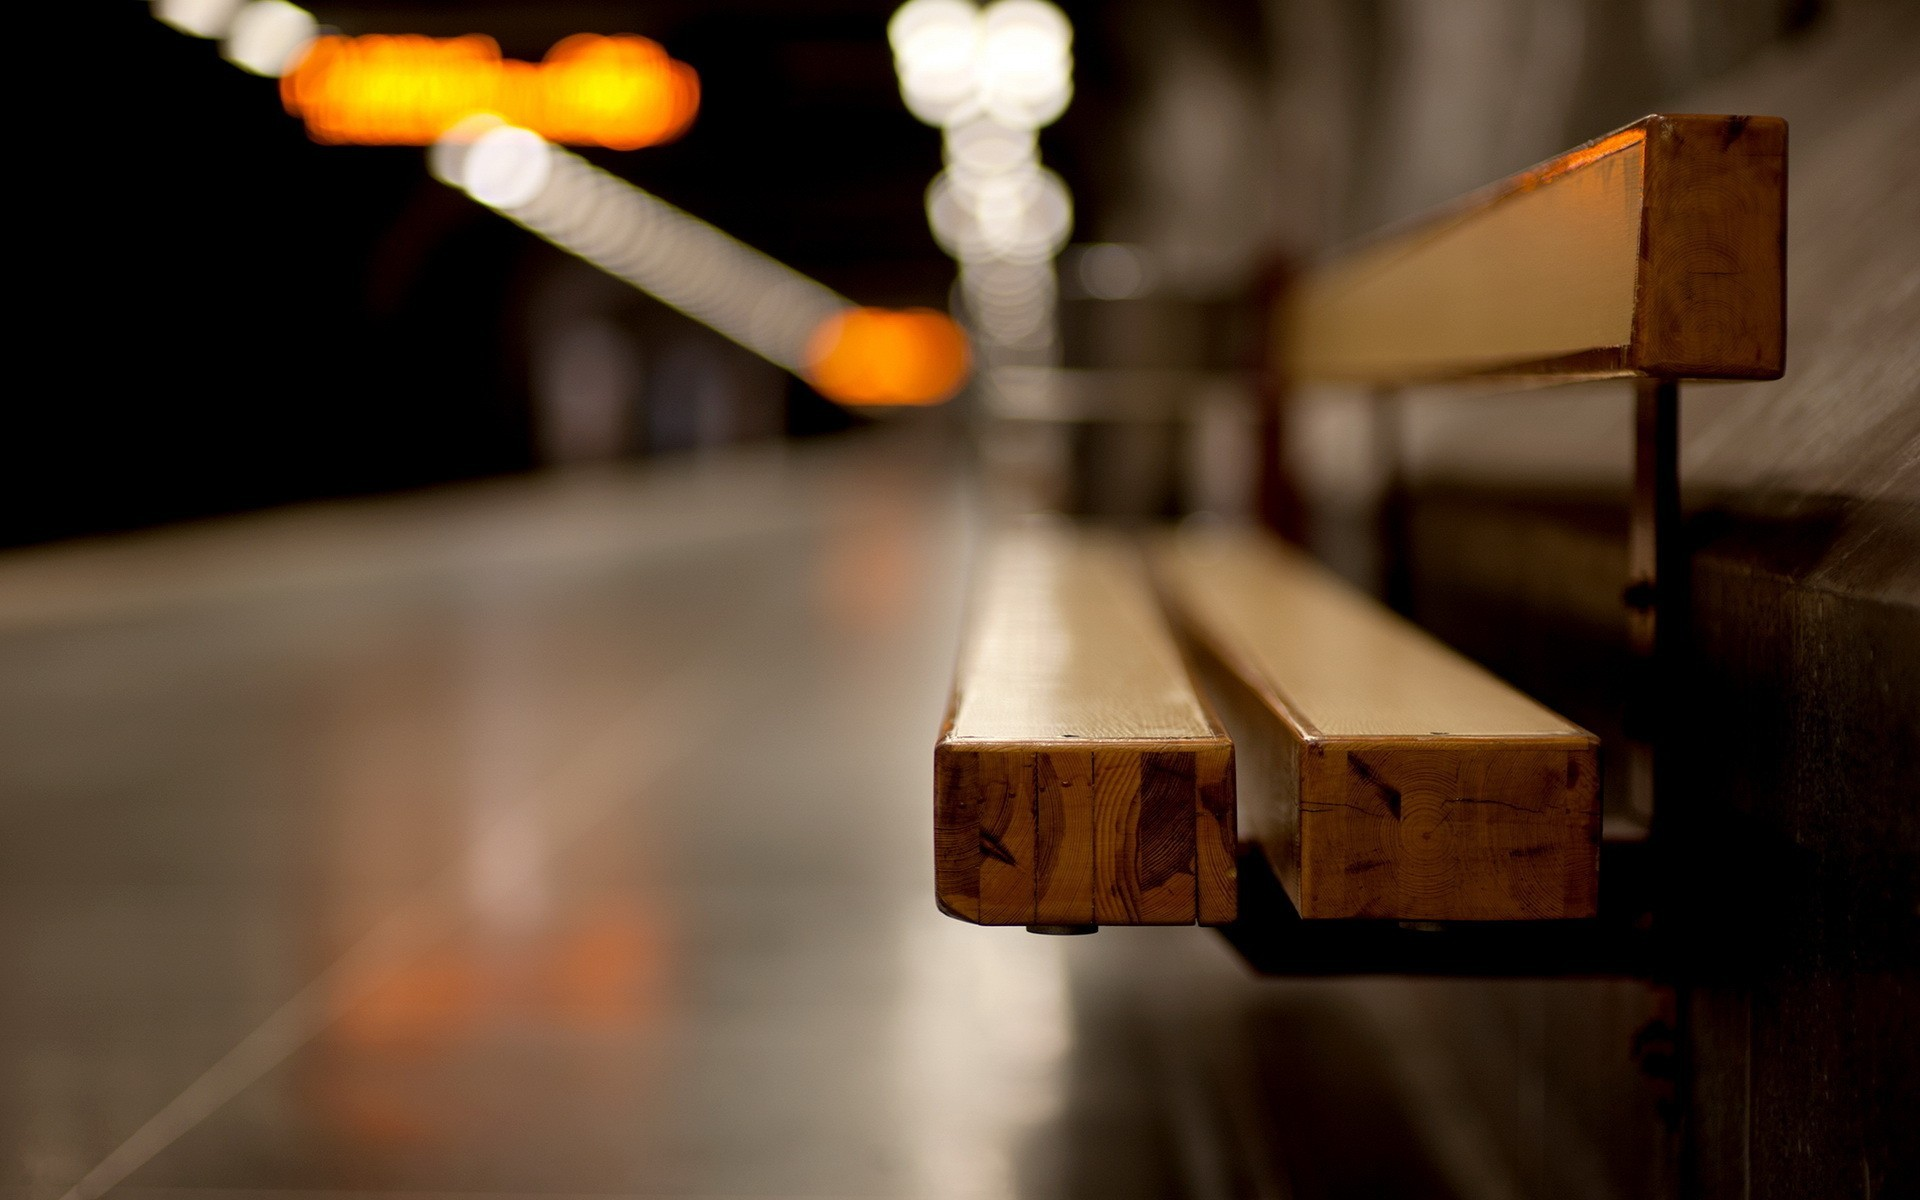
\includegraphics[width=\paperwidth,
                    height=\paperheight]{background}
}
\begin{frame}
\ \\ \ \\
\centering \Large \textcolor{white}{Q\&A}

\end{frame}
\usebackgroundtemplate{}
% ----------------------------------------------------------------------------


\end{document}
